 \chapter{Caso Estudio: Campus Universitario}
\label{chap:Caso Estudio: Campus Universitario}


En el presente proyecto se implementó una aplicación web móvil, como ya se explico, este tipo de aplicaciones son básicamente páginas web, con amplia funcionalidad e implementadas específicamente para su uso en dispositivos móviles, tablets o smartphones, para lo cual se investigó las tecnologías, arquitecturas y los frameworks de desarrollo que actualmente usan este tipo de aplicaciones, una de los concepto que se estudió fue de las \emph{aplicaciones de página única}, concepto que se empezó a discutir a principios de 2003, y se puso de moda con la aparición de frameworks JavaScript que agilizan y facilitan en gran medida la implementación de aplicaciones web, tales como  \emph{Angular.JS} y \emph{Backbone.JS} en el 2010 y \emph{Ember.JS}. \\

Es necesario reconocer las diferentes partes con la que cuenta una aplicación web móvil como una aplicación de página única diseñada para dispositivos móviles, es necesario implementar un REST API que se encargue de hacer las consultas a la base de datos y que el cliente pueda consumir la información obtenida de la base de datos así como también el camino inverso, la base de datos necesita manejar informacion geoespacial y el cliente necesita que la aplicación sea optimizada para su uso en dispositivos móviles. Tomando en cuenta estos requerimientos se puede separar el desarrollo del proyecto en los siguientes apartados. \\



\section{Generar el mapa con información geográfica}
\label{sec:generar_mapa_rutas}

Para poder responder al problema de encontrar una ruta optima entre 2 puntos dentro del campus universitario, se necesita de un mapa que contega todas las rutas que existen dentro del campus.\\

  %
  %
  % \section{Campus Universitario}
  % \label{sec:ruta_corta_umss}

  En primer lugar fue necesario obtener un grafo ponderado no-dirigido que represente un mapa de los caminos que existen dentro del campus Universitario.\\

  Para obtener este mapa se procedió a caminar a través del campus de la UMSS con un GPS Garmin Nuvi 1300\footnote{El Garmin Nuvi 1300, es un dispositivo GPS básico pero cumple con la funcion de guardar información geográfica, los archivos generados tienen extensión \emph{gpx}, el cual es básicamente un fichero XML estándar usado para compartir datos entre GPS's.}, se recorrieron los principales caminos que existen e interconectan las distintas facultades y oficinas dentro del campus universitario. Una vez realizado este recorrido, se procedió a extraer la información del dispositivo GPS, se utilizó el archivo \emph{current.gpx} para exportar la información  a un archivo \emph{shapefile}\footnote{Un shapefile es un archivo de formato sencillo y no topológico que se utiliza para almacenar la ubicación geométrica y la información de atributos de las entidades geográficas.\cite{what_is_shapefile} }, para esta tarea se utilizó QGis, con el cual se acabó editando las rutas recogidas por el GPS.\\

  Este paso fue necesario porque el mapa extraído del GPS es una línea única, pero para que nos sirva para el objetivo de buscar una ruta óptima, es necesario que esta línea sea dividida o separada en muchas líneas, las cuales son las aristas y los extremos de las líneas serán los nodos o vértices del grafo.\\

  Implementando el algoritmo de \emph{Dijkstra} en el grafo resultante es lo que nos permitir\'a encontrar la ruta más corta dentro del campus Universitario, al tener una gran cantidad de información resultante de la obtención de datos mediante un dispositivo GPS se hace imprescindible usar una base de datos que nos ayude con esta tarea, para lo cual se usó la base de datos PostgreSQL añadiendolo PostGIS y pgRouting, herramientas ampliamente utilizadas en el manejo de datos geo-espaciales.\\

   % el grafo representa el mapa de caminos  pueda ser usado en una base de datos  “ruteable”, esto significa que el mapa de una sola línea hay que separarlo o dividirlo en muchas líneas.\\


  Técnicamente esta línea única es representada como un \emph{POLYLINE} el cual consiste en una o más partes. Una parte es una secuencia conectada de dos o más puntos. Las partes pueden o no estar conectadas entre sí. Las partes pueden o no intersectarse entre sí, para transformar este POLYLINE necesitamos separar todas sus partes y convertirlas en objetos \emph{LINESTRING} únicos, y a este conjunto de LINESTRINGs es el que se va a usar en la base de datos como mapa de ``rutas''.\cite{esri_shapefile}\\

  \begin{figure}[H]
    \begin{center}
      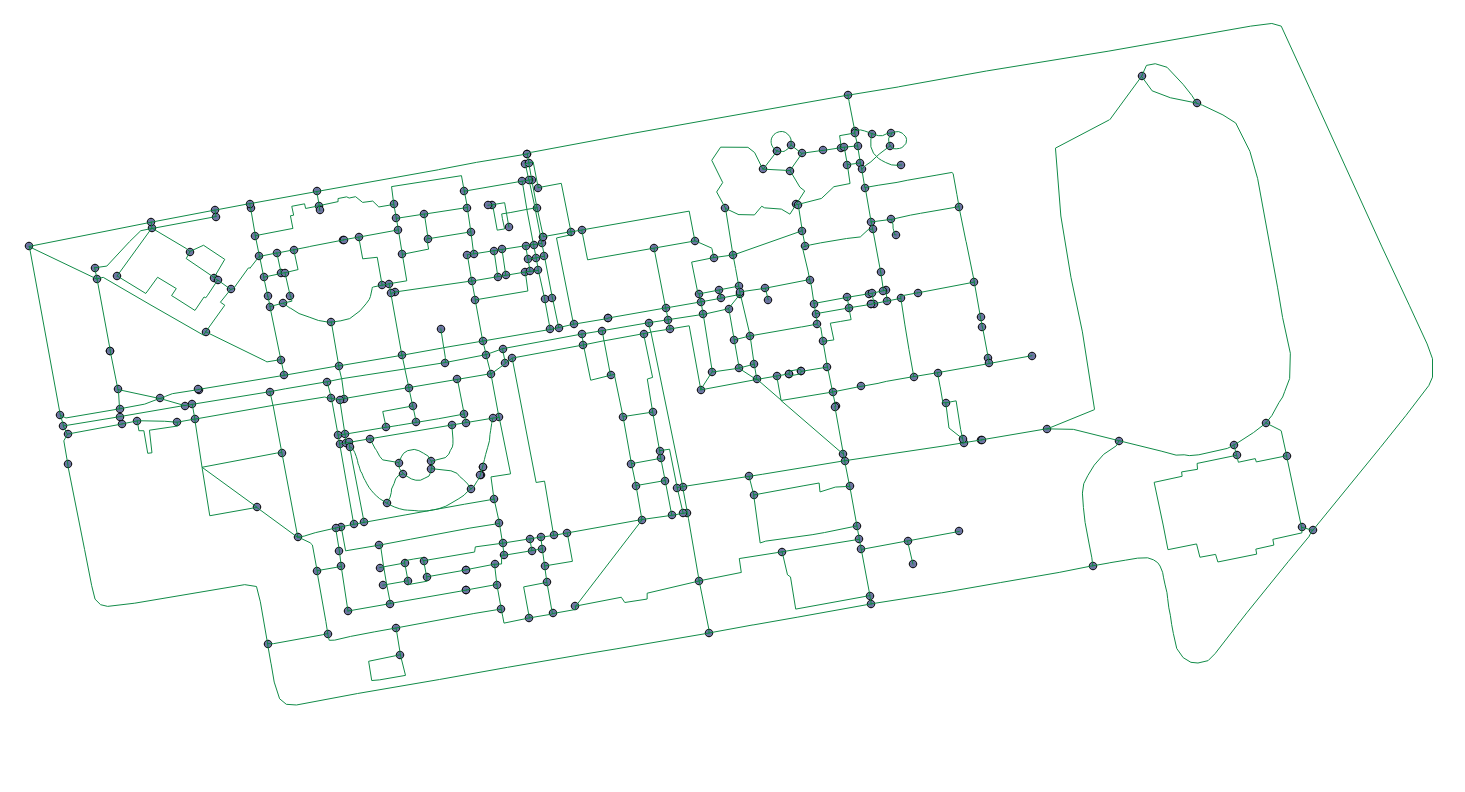
\includegraphics[width=1\textwidth]{shapefile_umss_v1}
      \caption{Shapefile del campus Universitario.}
      \label{fig:shapefile_umss_v1}
      \caption*{Fuente: Elaboración propia}
    \end{center}
  \end{figure}

  En la figura \ref{fig:shapefile_umss_v1} se puede apreciar el shapefile resultante de la división del POLYLINE original, las líneas que conforman el mapa de las rutas del campus Universitario, donde cada línea es una arista y los puntos son los nodos del grafo no-dirigido, que será usado para la resolución del problema de la ruta más corta en el presente proyecto de grado.\\

  Para una mejor apreciación del grafo que consta de 1164 aristas y 1003 vértices, se lo puede ver en combinación o proyectada en un mapa de rutas del campus de la Universidad Mayor de San Simón ubicado entre las calles Oquendo, Sucre y  Belzu de la ciudad de Cochabamba - Bolivia, se puede referir a la siguiente figura \ref{fig:shapefile_umss_v2}.

  \begin{figure}[H]
    \begin{center}
      \caption{Campus Universitario de la UMSS ubicado en la calle Oquendo, Cochabamba-Bolivia.}
      \label{fig:shapefile_umss_v2}
      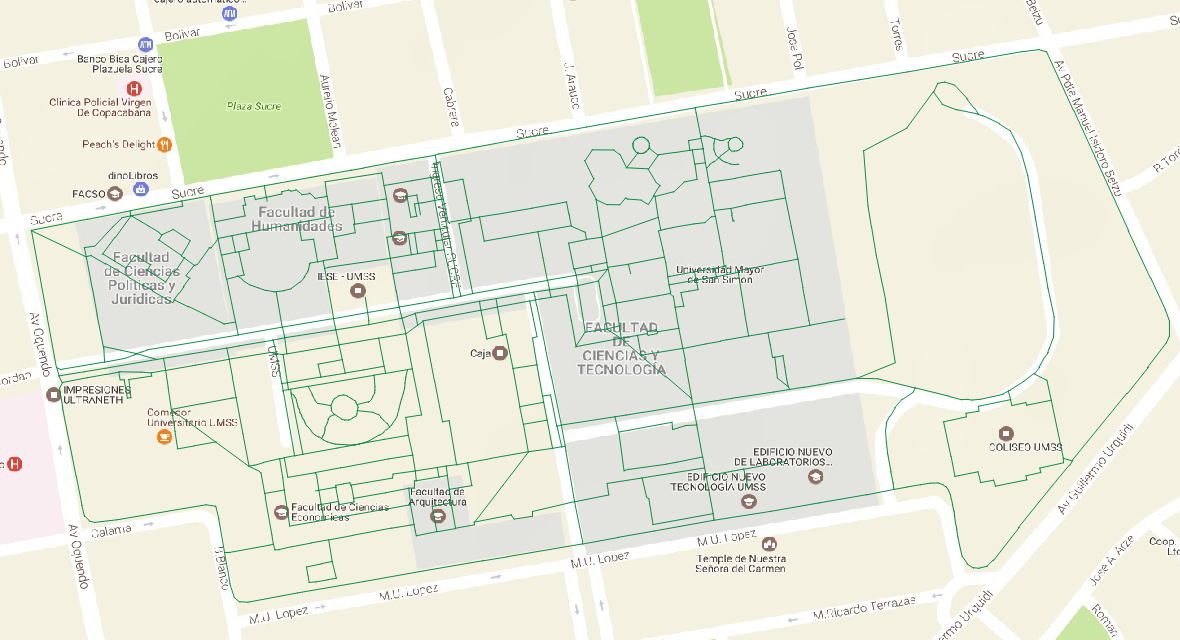
\includegraphics[width=1\textwidth]{shapefile_umss_v2}
      \caption*{Fuente: Elaboración propia}
    \end{center}
  \end{figure}


  \subsection{Facultad de Derecho}
  \label{sub:facultad_derecho}

  La facultad de Derecho cuenta con alrededor de 178 vértices y 88 aristas, está ubicada al nor-oeste del Campus Universitario, en la esquina de la calle Oquendo y Sucre, dentro del campus colinda con la facultad de Humanidades hacia el Nor-Este y hacia el Sur-Oeste está la facultad de Economía.

  \begin{figure}[H]
    \begin{center}
      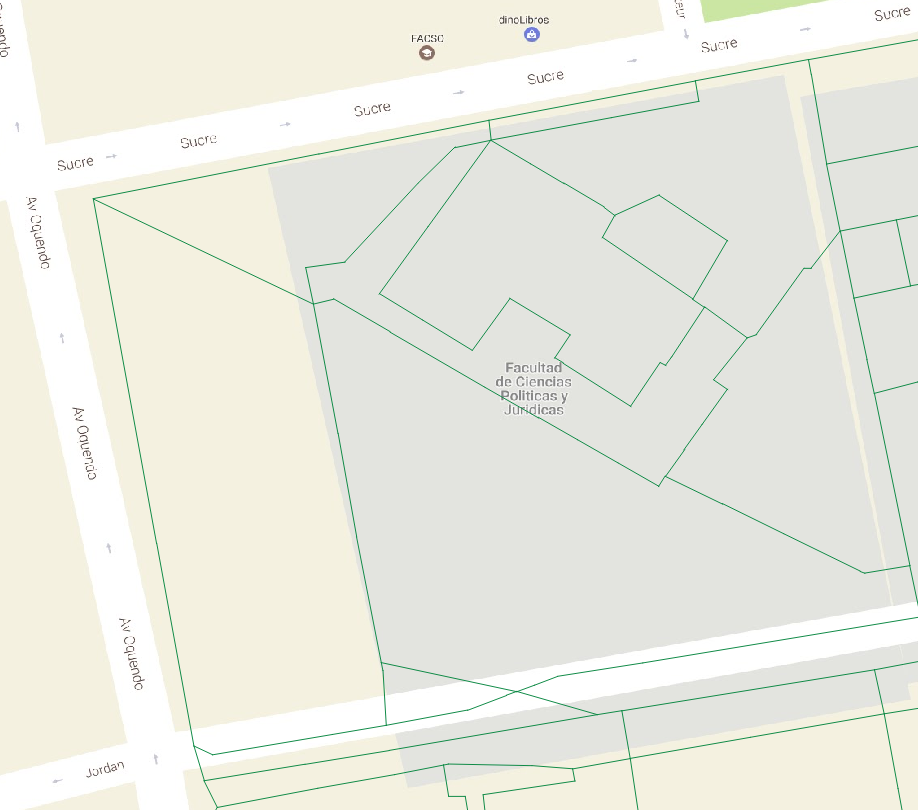
\includegraphics[width=0.75\textwidth]{fac_derecho}
      \caption{Facultad de Derecho - UMSS}
      \label{fig:fac_derecho}
      \caption*{Fuente: Elaboración propia}
    \end{center}
  \end{figure}

  En la figura \ref{fig:fac_derecho} se puede observar en la linea verde los caminos o rutas dentro de la facultad de derecho de la UMSS, proyectada sobre el mapa de Google Maps, para lograr esta representacion se utilizo QGIS ya que la informacion geografica de la ruta esta contenida en un archivo shapefile y el mapa se lo obtiene usando el API de Google Maps gracias al plugin de QGIS, \emph{QuickMapServices}\footnote{http://nextgis.com/blog/quickmapservices/}.


\subsection{Facultad de Economía}
\label{sub:facultad_economia}

La facultad de Economía está compuesta de XX aristas y XXX vértices, está ubicada en el sector Sur-Oeste del campus Universitario, colinda con las calles Oquendo y M. U. López, dentro del campus al Nor-Este se encuentra la facultad de Arquitectura y al Nor-Oeste la facultad de Derecho, tal como se puede apreciar en la figura \ref{fig:fac_economia}.

\begin{figure}[H]
  \begin{center}
    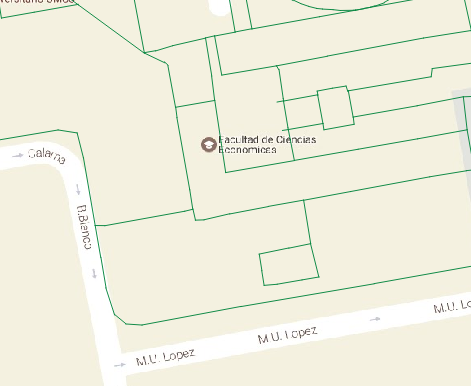
\includegraphics[width=0.75\textwidth]{fac_economia}
    \caption{Facultad de Economia - UMSS}
    \label{fig:fac_economia}
    \caption*{Fuente: Elaboración propia}
  \end{center}
\end{figure}



\subsection{Facultad de Humanidades}
\label{sub:facultad_humanidades}

La facultad de Humanidades está compuesta por XX aristas y XXX vértices, colinda con la calle Sucre hacia el Nor-Oeste, dentro del campus Universitario se encuentra la facultad de Tecnología hacia el Nor-Este, hacia el Sur-Oeste está la Facultad de Derecho y al Sur-Este se encuentra la Facultad de Arquitectura, en la figura \ref{fig:fac_humanidades} se puede apreciar la facultad de Humanidades dentro del campus Universitario sobrepuesto con el mapa de rutas identificado por la línea verde.

\begin{figure}[H]
  \begin{center}
    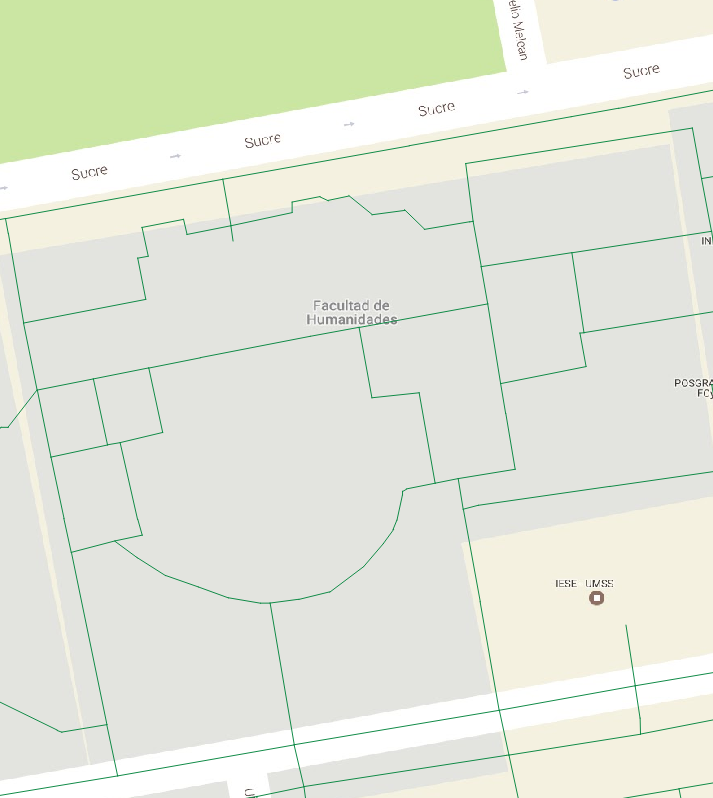
\includegraphics[width=0.75\textwidth]{fac_humanidades}
    \caption{Facultad de Humanidades - UMSS}
    \label{fig:fac_humanidades}
    \caption*{Fuente: Elaboración propia}
  \end{center}
\end{figure}


\subsection{Facultad de Tecnología}
\label{sub:facultad_tecnologia}

La facultad de Tecnología se encuentra en el extremo Nor-Este dentro del campus Universitario y cuenta con XX aristas y XXX vértices, la facultad de tecnología colinda hacia el Nor-Oeste con la calle Sucre, y hacia el Este con la calle Belzu, dentro del campus Universitario colinda con las facultades de Arquitectura y Humanidades que se encuentran hacia el Sur-Este y Sur-Oeste correspondientemente, en la siguiente figura \ref{fig:fac_tecno} se puede apreciar el mapa de rutas de la facultad de Tecnología.

\begin{figure}[H]
  \begin{center}
    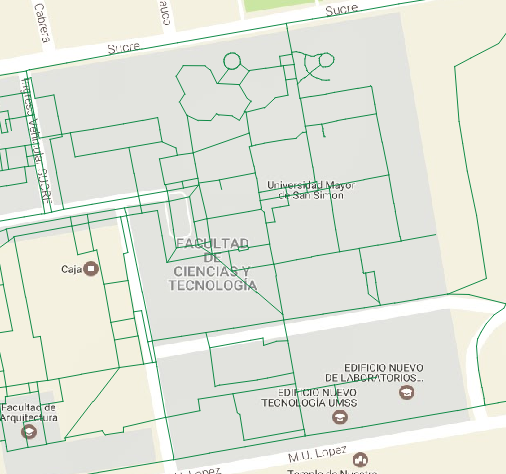
\includegraphics[width=0.75\textwidth]{fac_tecno}
    \caption{Facultad de Tecnologia - UMSS}
    \label{fig:fac_tecno}
    \caption*{Fuente: Elaboración propia}
  \end{center}
\end{figure}

\subsection{Facultad de Arquitectura}
\label{sub:facultad_arquitectura}

El grafo correspondiente a la facultad de Arquitectura cuenta con XX aristas y XXX vértices, la facultad colinda con la calle M. U. Lopez, dentro de los predios del campus Universitario se halla entre las facultades de Economía hacia el Sur-Este y con la facultad de Tecnología hacia el Nor-Oeste, el grafo se puede apreciar en la siguiente figura \ref{fig:fac_arqui}.

\begin{figure}[H]
  \begin{center}
    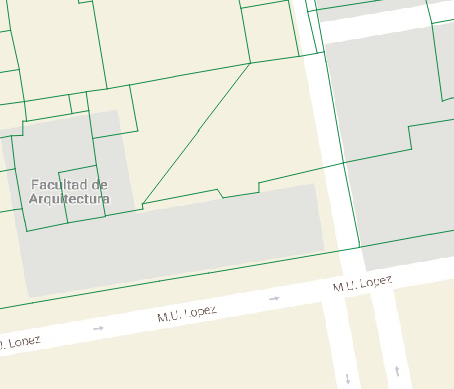
\includegraphics[width=0.75\textwidth]{fac_arqui}
    \caption{Facultad de Arquitectura - UMSS}
    \label{fig:fac_arqui}
    \caption*{Fuente: Elaboración propia}
  \end{center}
\end{figure}






\section{Backend}
\label{sec:Backend}

El backend de la aplicacion comprende el manejo de la informacion y como es procesada para su consumo por parte del frontend y almacenamiento en la base de datos, por lo tanto se pueden observar dentro del backend, 2 secciones claramente diferenciadas: el servidor web y la base de datos.\\




\subsection{Servidor Web}
\label{sub:servidor_web}

Un servidor web se puede referir a 2 cosas, la primera es la maquina en la cual se instalara y alojara toda la logica de negocio que requiere la aplicacion, la segunda se refiere a la capacidad de poder recibir y dar informacion al cliente del servidor, el segundo caso es tambien conocido como un \emph{servicio web} el cual sera discutido en esta seccon.\\

El servidor web es el encargado de enviar la pagina HTML la primera vez que el cliente hace un request al servidor, una vez que la pagina esta cargada el servidor solo se encarga de enviar y resivir informacion de la base de datos al cliente.\\

El servidor web sera construido con \emph{Express JS}, para lo cual primeramente se necesita instalar \emph{Node JS}, \emph{Express JS} cuenta con una herramienta para la consola, \emph{express-generator}, entonces solo es necesario crear un projecto Express y empezar a implementar la logica de negocio.\\

El servidor se va a encargar de hablar con la base de datos y tambien necesita ofrecer una interfaz por la cual pueda recibir datos y entregar datos, en pocas palabras un \emph{API}, implementar un \emph{API} con \emph{Express} es bastante sencillo, para trabajar con la base de datos se instalo una libreria \emph{Bookshelf.JS} para poder escribir las consultas y trabajar con la bd como si se tratara de objetos\footnote{Este patron se denomida ORM, Object-Relational-Model, basicamente mapea las tablas y las relaciones como objetos y el framework se encarga de traducirlo a lenguaje \emph{SQL} que es el lenguaje que entienden las bases de datos.} y tambien podemos escribir las consultas en lenguaje \emph{SQL}, si fuera necesario. Como en el presente caso ya que al  trabajar con una herramienta especifica, \emph{pgRouting}, las consultas son personalizadas.\\

% \begin{minted}{js}
  \begin{center}
    \begin{verbatim}
      var getPlace = (req, res) => {
        var id = req.params.id;
        var raw = "SELECT " +
                  " ST_AsGeoJSON(geom)::json As geometry," +
                  " name," +
                  " description," +
                  " phone," +
                  " level," +
                  " gid As id " +
                  " FROM place WHERE gid = " + id;
        Bookshelf.knex.raw(raw)
          .then((data) => {
            res.json(data.rows[0]);
        })
          .catch((error) => {
            console.log(error);
            res.send("Error");
        });
      };
    \end{verbatim}
  \end{center}
  %  \end{minted}

Como en la anterior consulta, se requiere obtener la informacion de un lugar, por lo tanto se necesita  usar la forma \emph{Raw SQL}\footnote{Raw SQL se refiere a consultas en ``SQL puro'' ya que el fuerte de \emph{Bookshelf.JS} es el manejo de las consultas en forma de objetos (ORM), lamentablemente actualmente no existe mucho soporte para manejar datos geospaciales}, de \emph{Bookshelf.JS}.
% De esta forma se obtiene de la base de datos la infor  donde este
Una vez que se obtiene la informacion del lugar; nombre, descripcion, telefono, el nivel o piso donde se encuentra pero lo importante de esta consulta es la obtencion del ``punto'' geoespacial del lugar. Estos datos son importantes para implementar la logica de negocio.\\


\begin{center}
  \begin{verbatim}
    "POINT (-66.14857015827988 -17.394421906929086)"
  \end{verbatim}
\end{center}

% var raw = "SELECT seq, id1 AS node, id2 AS edge, cost
%            FROM pgr_dijkstra('SELECT gid AS id,
%                                     source::integer,
%                                     target::integer,
%                                     st_length(geom) AS cost
%                               FROM public.ways', targetId, sourceId, false, false);";


 Este atributo es de tipo \emph{punto} o \emph{point} el cual tiene un \emph{SRID}\footnote{ Spatial Reference System Identifier, El \emph{SRID} corresponde a un sistema de referencia espacial basado en el elipsoide concreto usado para la creación de mapas de tierra plana o de tierra redonda.\cite{msdn_srid} } \emph{3857}\footnote{La proyeccion Mercator usa el EPSG 3857}, el SRID  es la llave primaria de la tabla \emph{spatial\_ref\_sys} que se crea cuando se inicializa una base de datos que soporte informacion geoespacial (PostGis), esta tabla provee la informacion necesaria para interpretar y convertir correctamente todas las coordenadas existentes, el \emph{SRID 3857} esta definida en la tabla \emph{spatial\_ref\_sys} como ``Popular Visualisation CRS / Mercator''.\\


En resumen el servidor web sera el encargado de recibir informacion y devolver una respuesta de acuerdo a los datos que recupere de la base de datos, para tal efecto se utilizan las direcciones URL, las cuales de acuerdo al protocolo HTTP se pueden definir de acuerdo a al accion que el servidor necesita procesar, para lograr esta comunicacion es necesario definir nuestro API.\\


\subsubsection{Implementacion del REST API}
\label{subs:Implementacion del REST API}



 El servidor necesita reconocer las peticiones que le llegan del cliente, para lo cual es neceario ``mapear'' un URI a una accion especifica, las cuales ya estan preparadas para comunicarse con la base de datos, no hay restriccion en la declaracion de las URIs pero para una mejor comprension del API que se esta desarrollando es necesario seguir convenciones que aseguran que cualquier desarrollador puedafloatpag comprender el API presentado y pueda ser facilmente consumido por cualquier aplicion que requiera aceder a la informacion que disponible, un API REST es el que cumple con estas caracteristicas.
 En primer lugar es necesario crear las URIs que seran ``entendidas'' por el servidor, esto se logra declarandolas en el servicio creado con \emph{Express.JS}, tal como se puede apreciar en el siguente bloque de codigo, cada URI se lo relaciona a un metodo en especifico de acuerdo a la accion que se requiere, tal como se puede observar en el cuadro \ref{tab:rest} las URIs declaradas en el API cumplen con tal caracteristica.\\


 % \begin{minted}{js}[label=express_api,caption=Declarando API REST con ExpressJS]
 \begin{center}
   \begin{lstlisting}[label=express_api,caption=Declarando API REST con ExpressJS]
         const router = express.Router();
         router.get('/', places.getAll);
         router.get('/:id', places.getPlace);
         router.post('/', places.newPlace);
         router.put('/:id', places.editPlace);
         router.delete('/:id', places.deletePlace);

         app.use('/api/v1/places', router);
   \end{lstlisting}
 \end{center}
 % \end{minted}

% En el codigo

   %
   % Para lograr todo este comportamiento  es necesario declarar, en el archivo
   % que controla las rutas dentro de la aplicación, \textbf{routes}, que el
   % recurso \textbf{user} es \emph{restful}, tal como se muestra en la figura \ref{fig:rest}\\

   % \begin{figure}[!hbp]
   %   \begin{center}
   %     \caption[REST - routes.rb]{config/routes.rb}
   %     \label{fig:rest}
   %     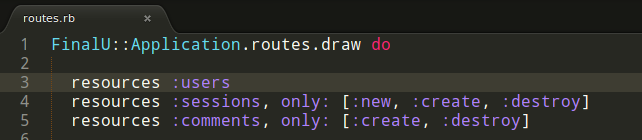
\includegraphics[width=1\textwidth]{rest}
   %     \caption*{Fuente: }
   %   \end{center}
   % \end{figure}

   El cuadro \ref{tab:rest} muestra como se puede leer las peticiones al API de \textbf{places}, las acciones mostradas son las que se pueden encontrar en un API REST pero no es necesario declaralas todas para considerar a que un API es restful.\\


   \begin{table}[!hbp]
     \begin{center}
       \caption[recursos REST]{REST URIs para los lugares}
       \label{tab:rest}

       \begin{tabularx}{0.75\textwidth}{ l l l  X }
         \toprule
         \multicolumn{1}{c}{\textbf{HTTP}} &
         \multicolumn{1}{c}{\textbf{URI}}  &
         % \multicolumn{1}{c}{\textbf{C}}  &
         \multicolumn{1}{c}{\textbf{ACCI\'ON}} &
         \multicolumn{1}{c}{\textbf{USADO PARA}}  \\
         \multicolumn{1}{c}{\textbf{request}} & & & \\

         \midrule
         GET     &  /places    &  index    & devuelve una lista con todos los lugares\\
         POST    &  /places    &  create   & inserta un nuevo lugar en la bd\\
         GET     &  /places/1  &  show     & muestra el lugar con identificador \emph{1}\\
         PUT     &  /places/1  &  update   & actualiza los datos de un lugar específico\\
         DELETE  &  /places/1  &  delete   & elimina el lugar con id = 1 de la bd\\
         \bottomrule
       \end{tabularx}

       \caption*{Fuente: Elaboracion propia}
     \end{center}
   \end{table}

   % Tal como se ve en el cuadro \ref{tab:rest}, Rails maneja los request HTTP de acuerdo con
   % el tipo de llamada que se realice, este trabajo lo realiza el \textbf{router},
   % que reconoce las URLs y los despacha a una \textbf{acción} del controlador,
   % todo este proceso ya está implementado en el núcleo de Rails por lo tanto  es automático y el programador
   % no necesita más configuración que la mostrada en la figura \ref{fig:rest},
   % obedeciendo al principio de \emph{Convención sobre configuración}\\

   % % no son más que métodos dentro del \emph{user\_controller.rb}
   % el cual
   % es parte del controlador de la arquitectura MVC.\\

   % The Rails router recognizes URLs and dispatches them to a controller’s action. It can also generate paths and URLs, avoiding the need to hardcode strings in your views.

   Por ejemplo, si se genera una petición GET hacia la direcci\'on
   \mbox{\emph{/places/1}}  el servidor interpreta la dirección y responde
   mostrando la información del lugar “1” y en cambio si se genera
   una petición PUT a la misma direcci\'on \emph{/places/1} se ejecuta la acción \textbf{update} y se actualizan los datos del lugar ``1''.

   % \textbf{usuarios} actualizando la información del usuario “1”. \\

   Siguiendo la convención de un API REST ayuda a entender el flujo que tiene un recurso,
   las URL son legibles y únicos para cada recurso. Por lo tanto la implementación   de los recursos se hace de forma más limpia y ordenada, situaciones que son   claves para el mantenimiento y la extensibilidad del sistema.




\subsection{La Base de Datos}
\label{sub:data_base}

      %
      % \subsection{Que se us\'o en la Aplicaci\'on} % (fold)
      % \label{sub:que_se_uso_en_la_aplicacion}
         Para preparar la base de datos es importante entender las diferencias entre los distintos tipos de sistemas de coordenadas porque computacionalmente realizar operaciones sobre los sistemas de coordenadas tiene un costo.\\

        Si se usara el sistema de coordenadas geográfico (WSG84) este es el más apropiado si se necesitaria usar grandes extensiones de la superficie terrestre, que al ser una estructura elipsoidal el costo computacional para realizar las operaciones matemáticas de calcular distancias, intersecciones, etc. es más elevado. En cambio el uso de un sistema de coordenadas proyectado (Mercator Projection) tiene un costo computacional más bajo, ya que se estaría trabajando con un sistema geométrico.\\

        % Por otro lado,
        También hay tomar en cuenta la base de datos, ya que será esta la que se encargara de manejar los datos espaciales. Al estar usando PostGIS, se puede ver que en su documentacion que claramente exorta el uso de un sistema geometrico sobre el uso de un sistema geografico si  se va trabajar con datos que cubran una pequena area geografica. Tomando en cuenta esta recomendacion y el tamano del área de estudio (el campus de la UMSS), se procedió a implementar en la base de datos el uso de la proyeccion Mercator. Se va usar Mercator sobre las otras proyecciones porque aparte de las ventajas que se mencionaron con anterioridad, Google Maps usa esta proyeccion y ya que se usara este mapa lo más correcto es trabajar con la misma proyeccion. \\

% \footnote{ http://postgis.org/documentation/manual-1.5/ch04.html} documentacion Postgis

        Toda la informacion geoespacial recolectada necesariamente debe ser almacenada, para lo cual se investigó las diferentes bases de datos disponibles y tras la tarea de investigar hacerca de ese problema se prosedio a instalar \emph{PostgreSQL 9.4.8} sobre Linux \emph{Ubuntu 15.10}, y para manejar datos geoespaciales se necesitó instalar \emph{PostGIS 2.1.8}.\\


        \subsubsection{Los lugares}
        \label{subs:Los lugares}

        En primer lugar se recolecto la informacion de los lugares, que la aplicacion contendra  de forma inicial, al igual que para recolectar las rutas se hizo uso de un \emph{GPS Garmin Nuvi 1300}, el cual cuenta con la opcion de guardar locaciones como favoritos, entonces solo fue necesario estar cerca del lugar que se desea guardar y activar esa opcion del GPS, este guarda la informacion en un archivo \emph{.gpx} y con la ayuda de \emph{QGIS} se genero el archivo shapefile correspondiente.\\

        Posteriormente es necesario pasar la informacion geoespacial del shapefile a la base de datos, para esta tarea se hizo uso de una herramienta disponible para postgres, \emph{shp2pgsql}, que permite la conversion de un archivo shapefile a un archivo sql.

        % $ shp2pgsql -s 4326 -I -S -c -d ~/Documents/places.shp > places.sql
        \begin{verbatim}
          $ shp2pgsql -s 3785 -I -S -c -d ~/Documents/places.shp > places.sql
        \end{verbatim}

        Con el anterior comando se tiene como resultado un archivo \emph{.sql}, el cual es ingresado en la base de datos ya configurada, de esta forma nuestra base de datos para a contener una tabla geoespacial con datos de tipo \emph{POINT}, los cuales representan los lugares dentro del campus de la UMSS.\\

        % \begin{verbatim}
        %   $ shp2pgsql -s 4326 -I -S -c -d ~/Documents/ways.shp > ways.sql
        % \end{verbatim}
        %
        % De la misma forma es necesario pasar la informacion de las rutas contenidas en un archivo shapefile a un archivo sql, en este caso creara una tabla \emph{WAYS}.\\

        El archivo \emph{sql} resultante es usado para popular la base de datos con la informacion inicial de los lugares que contiene el campus universitario, para tal tarea se uso el siguiente comando.\\
        % Los archivos resultantes \emph{sql} son usados para popular la base de datos .\\

        \begin{verbatim}
          $ psql -d db_ubikate -U db_admin -f /Documents/places.sql
        \end{verbatim}

        \begin{figure}[H]
          \begin{center}
            \caption{Herramienta grafica de PostgreSQL (pgAdmin) con la tabla de Lugares desplegada.}
            \label{fig:postgres_places}
            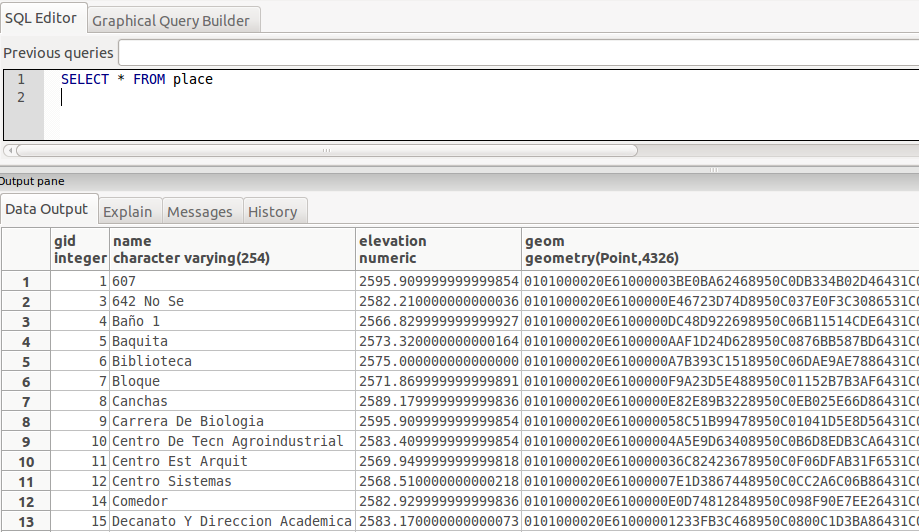
\includegraphics[width=1\textwidth]{iteration1/postgres_places}
            \caption*{Fuente: Elaboración propia}
          \end{center}
        \end{figure}

        En la figura \ref{fig:postgres_places} se puede observar que la columna \emph{Elevation} contiene datos que el GPS Garmin Nuvi 1300 genera al momento de guardar un punto, en el presente caso es irrelevante.\\

        \subsubsection{Las Rutas}
        \label{subs:Las Rutas}

        Despues de generar un archivo shapefile en la secion \ref{sec:generar_mapa_rutas}, se procede a popular la base de datos del mismo modo que se hizo con la informacion de los lugares. Para las rutas se genera una tabla nombrada \emph{ways}.\\

        Posteriormente se procede a preparar la tabla \emph{ways} para que soporte las funciones instaladas por pgRouting.
        % Una vez populada la base de datos se procede a cargar la misma con la informacion obtenida en RF011, para tal efecto es necesario primeramente crear una tabla que contendra los LINESTRING contenidos en el shapefile, esta operacion es similar a la realizada en la tarea - RF003 (\ref{sub:RF003}). Una vez que ya se tiene la tabla a la llamamos \emph{ways},
        Es necesario ejecutar un query propio de \emph{pgRouting} el cual tiene como objetivo analizar los datos geo-espaciales de la tabla y a\~nadirle una \emph{topologia}.\\

        \begin{verbatim}
          select pgr_createTopology('ways', 0.00000001, 'geom', 'gid');
        \end{verbatim}

        Dentro lo que es la \emph{topologia geoespacial} existe una aplicacion que se lo conoce como \emph{topología de red}. La \emph{topología de red} representa las relaciones entre segmentos en una red lineal o una colección de segmentos de línea. \cite{osgeo_journal_topology} \\

        En un \emph{SIG} la topologia ayuda a mejorar el analisis de datos geo-espaciales, para resolver el problema de la ruta corta \emph{pgRouting} genera una \emph{topología de red} usando los datos que existen en la tabla \emph{ways}, es necesario ejecutar una instruccion, la que se muestra a continiacion y \emph{pgRouting} se encarga de llenar los datos que se pueden observar en la figura \ref{fig:postgres_ways}, las columnas \emph{source} y \emph{target} son populadas con el analisis topologico y en la figura \ref{fig:postgres_vertices}, se puede observar que la tabla \emph{ways\_vertices\_pgr} es creada enteramente en la ejecucion de la instruccion.\\

        \begin{figure}[H]
          \begin{center}
            \caption{Vista de la tabla \emph{ways} en la base de datos PostgreSQL.}
            \label{fig:postgres_ways}
            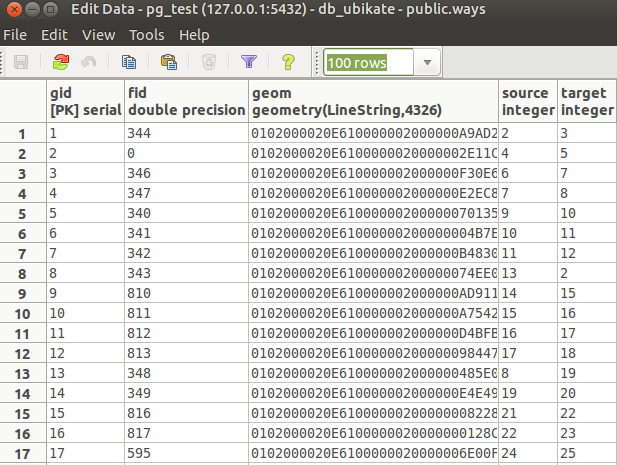
\includegraphics[width=1\textwidth]{iteration2/postgres_ways}
            \caption*{Fuente: Elaboración propia}
          \end{center}
        \end{figure}

        En la figura \ref{fig:postgres_ways} se puede apreciar que cada fila es una parte de la línea original obtenida por el dispositivo GPS y explisionada por QGIS, hay que notar que las columnas \emph{source} y \emph{target} hacen referencia a los nodos o vertices que la primera linea tiene en sus extremos, la primera linea o fila esta identificada por la columna \emph{gid}.\\

        En la siguiente figura \ref{fig:postgres_vertices} se observa la tabla \emph{ways\_vertices\_pgr} que contiene los vertices creados a partir del analisis de los datos en la tabla \emph{ways}.

        \begin{figure}[H]
          \begin{center}
            \caption{Vista de la tabla \emph{ways\_vertices\_pgr} en la base de datos PostgreSQL.}
            \label{fig:postgres_vertices}
            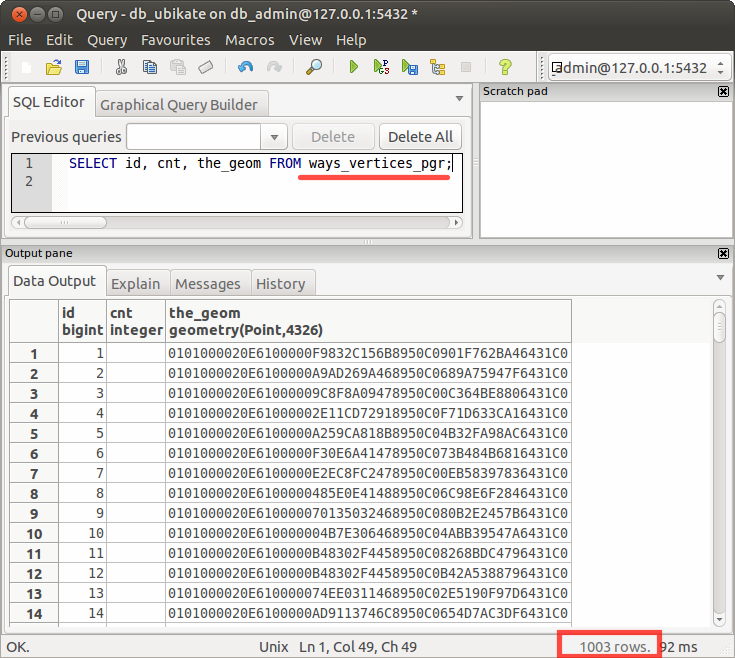
\includegraphics[width=1\textwidth]{iteration2/postgres_vertices}
            \caption*{Fuente: Elaboración propia}
          \end{center}
        \end{figure}

        Para entender los datos generados hay leer la informacion de las 2 tablas, por ejemplo en la primera  fila (gid 1) de la tabla \emph{ways}, se observa que el contenido de la columna \emph{source} es igual a \textbf{2} y \emph{target} es igual a \textbf{3}, eso quiere decir que los vertices del LINESTRING de la fila 1 son los vertices con \textbf{id} 2 y 3 respectivamente de la tabla \emph{ways\_vertices\_pgr}.\\


        Todo el conjunto de vertices y lineas de estas tablas se podria representar con una Matriz de adyacencias, explicada en \ref{sub:representacion_de_un_grafo}, y usada en la resolucion de la ruta mas corta, mas especificamente con el algoritmo de Dijkstra.\\

        \begin{center}
          \begin{lstlisting}[label=pgr_dijkstra,caption=Algoritmo de Dijkstra implementado en \emph{pgRouting}]
            SELECT seq, id1 AS node, id2 AS edge, cost
            FROM pgr_dijkstra(SELECT gid AS id,
                                      source::integer,
                                      target::integer,
                                      st_length(geom) AS cost
                               FROM public.ways, targetId, sourceId, false, false);
          \end{lstlisting}
        \end{center}


        La anterior consulta SQL es una llamada al metodo \emph{pgr\_dijkstra} implementado en \emph{pgRouting} el cual solo puede ser utilizado una vez que la base de datos esta preparada para tal efecto, es decir necesitamos que la tabla de rutas \emph{ways} tenga la topologia de red y tambien es necesario los ids de los nodos de destino y origen, \emph{targetId} y \emph{sourceId} respectivamente, estos dos ultimos datos son obtenidos por una combinacion de acciones ya que los nodos son propios del mapa de rutas y el punto destino es en realidad un lugar el cual esta ubicado en otra tabla y el punto origen es donde se encuentra el cliente dentro del campus Universitario, por lo tanto una vez obtenido los punto geo-referenciados del lugar de la tabla \emph{places} y el punto donde se encuentra parado el cliente se obtienen los nodos ``mas'' cercanos a estos puntos, gracias a que \emph{PostGIS} ya lo tiene implementado, encontrar el nodo mas cercano es tan facil como ejecutar la siguiente consulta SQL, donde \emph{lon} y \emph{lat} son la longitud y latitud del lugar.

        \begin{verbatim}
            SELECT id
            FROM ways_vertices_pgr
            ORDER BY the_geom <-> ST_GeometryFromText('POINT(lon lat)', 4326)
            LIMIT 1
        \end{verbatim}

        Una vez ejecutado el metodo \emph{pgr\_dijkstra} se obtiene un conjunto de lineas, que son un conjunto de latitudes y longitudes que representan la ruta mas corta entre el punto origen y el punto destino, esta informacion realmente no dice nada a la persona que lo lee por lo tanto requiere ser procesada para poder ser consumida desde el navegador, este proceso es llevada a cabo en el servidor y entregada al cliente en formato GeoJSON.\\


        % En la figura XX, se puede ver la tabla \emph{WAYS} con las rutas generadas.





        % Comoprojected
        % PostGIS maneja dos tipos de datos, geograficos y geometricos

      % section que_se_uso_en_la_aplicacion (end)
  % section sistema_de_coordenadas_para_datos_geograficos (end)
  % \section{Tipo de archivos} % (fold)
  % \label{sec:tipo_de_archivos}
  %
  % section tipo_de_archivos (end)

  % \subsection{Implementaci\'on} % (fold)
  % \label{sub:Implementacion}


    % Para menenjar datos georreferenciados con tecnologia JavaScript, ya que se implemento el Backend con NodeJS, se hizo uso del la libreria \textbf{KnexJS} para manejar la conecion a la base de datos PostgreSQL, y BookshelfJS para las consultas SQL pero para las conultas con datos geospaciales se realizo a traves de esta herramienta pero usando la forma \emph{Raw SQL}\footnote{Raw SQL se refiere a consultas en ``SQL puro'' ya que el fuerte de BookshelfJS es el manejo de las consultas en forma de objetos (ORM), lamentablemente actualmente no existe mucho soporte para manejar datos geospaciales}.


% Para implementar la comunicacion con la base de datos se

% El proyecto

% La estructura de archivos dentro del proyecto \emph{Express} se puede observar en la figura \ref{fig:express_structure}, donde se puede observar las secciones principales de routing, que se encarga de direccionar las peticiones web de acuerdo del protocolo HTTP, la seccion de \emph{views} donde estan los templates

% \begin{figure}[H]
%   \begin{center}
%     \caption[Express Aplication Structure]{Estructura de archivos de una Aplicacion \emph{Express}}
%     \label{fig:express_structure}
%     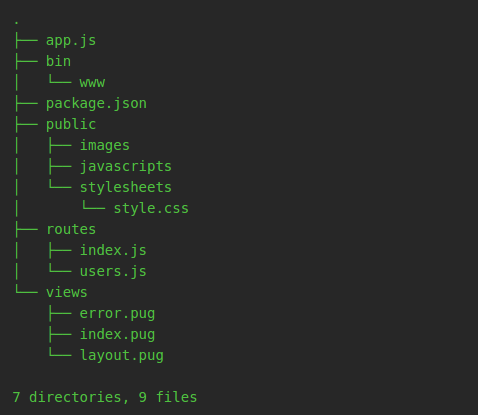
\includegraphics[width=1\textwidth]{express_structure}
%     \caption*{Fuente: https://expressjs.com}
%   \end{center}
% \end{figure}

% Dentro del proyecto \emph{Express} definimos una seccion donde localizamos la connecion y las consultas a la base de datos, y otra seccion donde



  %
  % Para menenjar datos georreferenciados con tecnologia JavaScript, ya que se implemento el Backend con NodeJS, se hizo uso del la libreria \textbf{KnexJS} para manejar la conecion a la base de datos PostgreSQL, y BookshelfJS para las consultas SQL pero para las conultas con datos geospaciales se realizo a traves de esta herramienta pero usando la forma \emph{Raw SQL}\footnote{Raw SQL se refiere a consultas en ``SQL puro'' ya que el fuerte de BookshelfJS es el manejo de las consultas en forma de objetos (ORM), lamentablemente actualmente no existe mucho soporte para manejar datos geospaciales}.
  %
  % \begin{center}
  %   \begin{verbatim}
  %     var raw = "SELECT " +
  %                 " ST_AsGeoJSON(geom)::json As geometry," +
  %                 " name," +
  %                 " description," +
  %                 " phone," +
  %                 " level," +
  %                 " gid As id " +
  %               " FROM place WHERE LOWER(name)
  %                      like LOWER('%" + name + "%')";
  %   \end{verbatim}
  % \end{center}

  % De esta forma es que se recupera de la base de datos un lugar georreferenciado, donde este tiene un nombre, una descripcion, un telefono, el nivel o piso donde se encuentra pero lo importante de esta consulta es la obtencion del ``punto'' geoespacial del lugar.
  %
  % \begin{center}
  %   \begin{verbatim}
  %     "POINT (-66.14857015827988 -17.394421906929086)"
  %   \end{verbatim}
  % \end{center}
  %
  % % var raw = "SELECT seq, id1 AS node, id2 AS edge, cost
  % %            FROM pgr_dijkstra('SELECT gid AS id,
  % %                                     source::integer,
  % %                                     target::integer,
  % %                                     st_length(geom) AS cost
  % %                               FROM public.ways', targetId, sourceId, false, false);";
  %
  %
  %  Este atributo es de tipo \emph{punto} \'o \emph{point} el cual tiene un \emph{SRID}\footnote{ Spatial Reference System Identifier, El \emph{SRID} corresponde a un sistema de referencia espacial basado en el elipsoide concreto usado para la creación de mapas de tierra plana o de tierra redonda.\cite{msdn_srid} } \emph{3857}\footnote{La proyeccion Mercator usa el EPSG 3857}, el SRID  es la llave primaria de la tabla \emph{spatial\_ref\_sys} que se crea cuando se inicializa una base de datos que soporte informacion geoespacial (PostGis), esta tabla provee la informaci\'on necesaria para interpretar y convertir correctamente todas las coordenadas existentes, el \emph{SRID 3857} esta definida en la tabla \emph{spatial\_ref\_sys} como ``Popular Visualisation CRS / Mercator''.\\


  Obtener la coordenada es el primer paso, seguidamente se debe mostrarlo sobre un mapa, en este caso \emph{Open Street Maps}, como se puede apreciar en la figura \ref{fig:ember_leaflet}, esta interfaz esta implementada usando \emph{ember-leaflet}, el cual esta principalmente dise\~nada para ofrecer una mejor experiencia de usario en celulares smartphones.\\

  % \begin{center}
  %   \begin{verbatim}
  %     var maker = new google.maps.Marker({
  %       position: new google.maps.LatLng( lat, lng  )
  %       map: UMSS.map
  %     });
  %   \end{verbatim}
  % \end{center}

  \begin{verbatim}
    {{#leaflet-map lat=lat lng=lng zoom=zoom}}
      {{tile-layer url="http://{s}.tile.openstreetmap.fr/hot/{z}/{x}/{y}.png" }}
        {{#marker-layer location=location}}
          <h3>{{model.name}}</h3>
          {{model.description}} <br>
          <strong>telf:</strong> {{model.phone}} <br>
          <strong>piso </strong>#{{model.level}}
      {{/marker-layer}}
    {{/leaflet-map}}
  \end{verbatim}

  \begin{figure}[H]
        \begin{center}
          \caption{\emph{ember-leaflet} nos ayuda a despleyar un mapa y mostrar un \emph{punto} o \emph{lugar} con un \emph{marcador} y dibuja una línea de color rojo sobre el mapa.}
          \label{fig:ember_leaflet}
          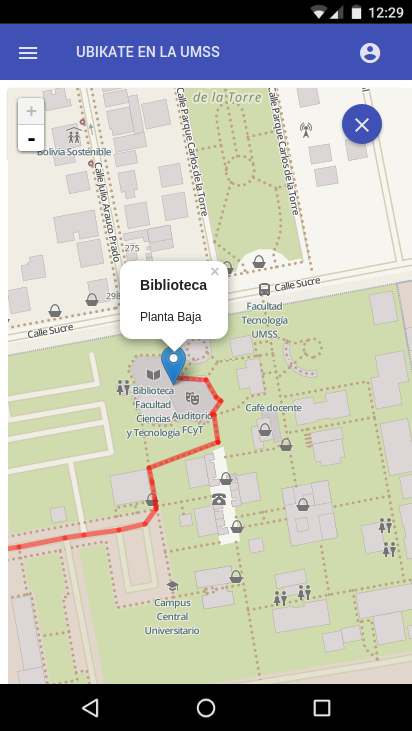
\includegraphics[width=0.5\textwidth]{ember_leaflet}
        \end{center}
        \caption*{Fuente: Elaboración propia.}
  \end{figure}


\section{Crear el Frontend}
\label{sec:Crear el Frontend}


El frontend como ya se menciono es la vista de la aplicacion, es donde el usuario interactua con la aplicacion, en el presente proyecto se implemento usuando \emph{Ember.JS}, el cual es un framework de desarrollo JavaScript orientado a crear Aplicaciones de Pagina Unica, esto quiere decir que una ves que se carge la pagina la primera vez ya no se recargara la pagina como tal, en cambio se actualizara de acuerdo como el usuario interactua con la aplicacion.\\

Ya que el proyecto se enfocara en la creacion de una aplicacion web optimizada para su uso en celulares, es primordial que el ``look and feel'' de la apliacion sea lo mas parecido a una aplicacion movil nativa, para lograr este efecto se utilizo \emph{ember-paper}, que ya trae implementado componentes (botones, listas, links, menus de navegacion, etc.) con un comportamiento que emula a una aplicacion movil nativa.\\

% Para empezar esta tarea se procedió a instalar y configurar el framework de desarrollo Ember JS, que nos ayudará en la implementación del frontend de la aplicación o la capa que interactúa con el usuaria, y Express JS, el cual manejara el backend de la aplicación, básicamente se encarga de la lógica del sistema y la comunicación con la base de datos.\\

\emph{EmberJS} esta basado en ``Convecion sobre Configuracion'', ya que la gran mayoria de los problemas con que uno se puede enfrentar a la hora de crear una aplicacion web ya fueron resueltas por la comunidad de desarrollo, por lo tanto ya se llego a un patron o convencion de como se deberia resolver algun determinado problema, \emph{EmberJS} implementa y sugiere soluciones a problemas comunes, para que de esa forma el desarrollo no se enfoque  en resolver problemas ya resueltos (configuracion) si no en implementar en la logica del negocio de la aplicacion, que al final es lo que le da valor al producto que queremos desarrollar y tambien para que si en un futuro otro desarrollador empieza a trabajar en el proyecto, sea capaz de entender la estructura y el diseno de la aplicacion de forma sencilla. Por lo tanto nos enfocaremos en analizar como se resolvieron los problemas: de como mostrar los lugares, geolocalizar el lugar sobre un mapa, mostrar la ruta mas corta dentro del campus Universtario, manejo de los usuario y como mostrar el reporte de los lugares mas visitados.

\subsection{Mostrar los Lugares}
\label{sub:Mostrar los Lugares}




%
% Para empezar esta tarea se procedió a instalar \emph{Ember.JS}, que al ser un paquete \emph{Node.JS} solo es necesario ejecutar el siguiente comando.
%
% \begin{verbatim}
%   $ npm install -g ember-cli
% \end{verbatim}
%
% Posteriormente se puede observar


Durante la investigacion de esta tarea se encontro \emph{ember-leaflet}, una libreria o plugin que contiene las herramientas para poder cargar y usar un servicio de mapas.\\

Para instalar esta libreria solo se necesita ejecutar el siguiente comando y posteriormente ya se puede empezar a utilizarla.\\

\begin{verbatim}
  $ ember install ember-leaflet
\end{verbatim}

El resultado de la investigacion puede apreciar en el marco teórico, en la sección que describe la librería, \emph{ember-leaflet}. \ref{sec:ember_js}





\begin{figure}[H]
  \begin{center}
    \caption{Vista de la lista de Lugares registrados en el sistema.}
    \label{fig:places_index}
    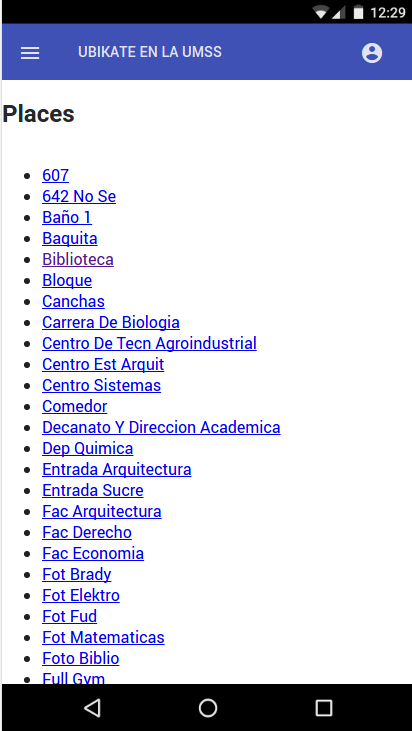
\includegraphics[width=0.5\textwidth]{iteration1/places_index}
    \caption*{Fuente: Elaboración propia}
  \end{center}
\end{figure}


\begin{figure}[H]
  \begin{center}
    \caption{Vista de la búsqueda de lugares a través de un cajón de búsqueda.}
    \label{fig:places_search}
    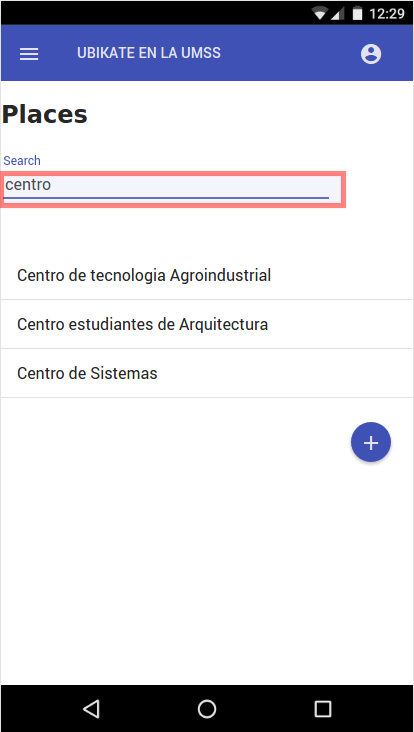
\includegraphics[width=0.5\textwidth]{iteration1/places_search}
    \caption*{Fuente: Elaboración propia}
  \end{center}
\end{figure}


Para implementar esta funcionalidad del sistema fue necesario utilizar las funcionalidad de Ember JS.

\begin{verbatim}
  {{#paper-item class="md-1-line" onClick=(transition-to 'places.show' place)}}
      <div class="md-list-item-text">
          <span>{{place.name}}</span>
      </div>
  {{/paper-item}}
\end{verbatim}


\begin{figure}[H]
    \label{fig:place_show}
    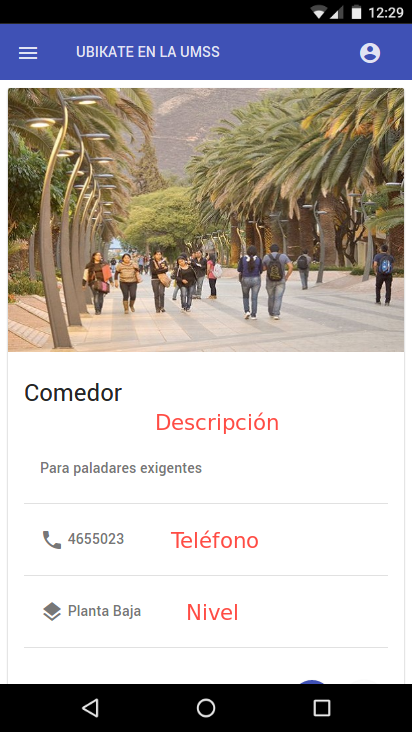
\includegraphics[width=0.5\textwidth]{iteration1/place_show}
    \caption*{Fuente: Elaboración propia}
  \end{center}
\end{figure}





\subsection{Mostrar los Rutas}
\label{sub:Mostrar los Rutas}


\subsection{Manejo de Usuarios}
\label{sub:Manejo de Usuarios}



\section{Informe de los datos}
\label{sec:Informe de los datos}
